%input macros (i.e. write your own macros file called MacroFile1.tex)
%\newcommand{\PdfPsText}[2]{
  \ifpdf
     #1
  \else
     #2
  \fi
}

\newcommand{\IncludeGraphicsH}[3]{
  \PdfPsText{\includegraphics[height=#2]{#1}}{\includegraphics[bb = #3, height=#2]{#1}}
}

\newcommand{\IncludeGraphicsW}[3]{
  \PdfPsText{\includegraphics[width=#2]{#1}}{\includegraphics[bb = #3, width=#2]{#1}}
}

\newcommand{\InsertFig}[3]{
  \begin{figure}[!htbp]
    \begin{center}
      \leavevmode
      #1
      \caption{#2}
      \label{#3}
    \end{center}
  \end{figure}
}


%%% Local Variables: 
%%% mode: latex
%%% TeX-master: "~/Documents/LaTeX/CUEDThesisPSnPDF/thesis"
%%% End: 


 \documentclass[oneside,12pt]{Classes/CUEDthesisPSnPDF}


\ifpdf
    \pdfinfo { /Title  (QoS-Aware Routing in Future All-IP Access Networks)
               /Creator (Alexandre Jaron)
               /Producer (Alexandre Jaron)
               /Author (Alexandre Jaron alexandre.jaron@kcl.ac.uk)
               /CreationDate (D:20140713000000)  %format D:YYYYMMDDhhmmss
               /ModDate (D:20030815213532)
               /Subject (Writing a PhD thesis in LaTeX)
               /Keywords (PhD, Thesis)}
    \pdfcatalog { /PageMode (/UseOutlines)
                  /OpenAction (fitbh)  }
\fi

\title{QoS-Aware Routing in Future \\
        All-IP Access Networks}

\ifpdf
  \author{\href{mailto:alexandre.jaron@kcl.ac.uk}{Alexandre Jaron}}
  \collegeordept{\href{http://www.kcl.ac.uk/nms/depts/informatics/research/telecomms/}{Centre for Telecommunications Research}}
  \university{\href{http://www.kcl.ac.uk}{King's College London}}
% insert below the file name that contains the crest in-place of 'UnivShield'
  \crest{
\includegraphics[width=35mm,height=30mm, trim= 10mm 8mm 12mm 12mm]{kcllogo}}
\else
  \author{Alexandre Jaron}
  \collegeordept{Centre for Telecommunciations Research}
  \university{King's College London}
% insert below the file name that contains the crest in-place of 'UnivShield'
  \crest{
\includegraphics[bb = 0 0 292 336, width=30mm]{kcllogo}}
\fi
%
% insert below the file name that contains the crest in-place of 'UnivShield'
% \crest{\IncludeGraphicsW{UnivShield}{40mm}{14 14 73 81}}
%
\renewcommand{\submittedtext}{A thesis submitted to King's College London in partial fulfilment of the requirements for the degree of}
\degree{Doctor of Philosophy}

\degreedate{February 2015}

% turn of those nasty overfull and underfull hboxes
\hbadness=10000
\hfuzz=50pt

% Put all the style files you want in the directory StyleFiles and usepackage like this:
\usepackage{StyleFiles/watermark}

% Comment out the next line to get single spacing
\onehalfspacing

% To insert a blank page
\usepackage{afterpage}
\newcommand\blankpage{%
    \null
    \thispagestyle{empty}%
    \addtocounter{page}{-1}%
    \newpage}

\begin{document}

%\language{english}

% A page with the abstract on including title and author etc may be
% required to be handed in separately. If this is not so, then comment
% the below 3 lines (between '\begin{abstractseparte}' and 
% 'end{abstractseparate}'), normally like a declaration ... needs some more
% work, mind as environment abstracts creates a new page!
% \begin{abstractseparate}
%   
% Thesis Abstract -----------------------------------------------------


%\begin{abstractslong}    %uncommenting this line, gives a different abstract heading
\begin{abstracts}        %this creates the heading for the abstract page

The proliferation of mobile devices over the past several years has created a whole new world of the Internet. The deluge of applications for every aspect of today�s life has raised the expectation of having ubiquitous connectivity, with a desired Quality of Service (QoS).  Although appealing, it has violated the original Internet design which was not intended to support mobility, neither better than best-effort delivery.

    It is also a well-known fact that technology is an ever-advancing need of the human society, and undeniably the Internet forms a major part of our lives now. Everyday more and more users flood the Internet with enormous amount of data and information. As such there is a need to effectively handle all the information and traffic in a way that there is an availability of high speed network routing without any loss in data transmission. 

     QoS provisioning has been one of the long lasting focuses in the network research community. While designed for fixed networks, the use of QoS protocols in IP-based mobile networks, where hosts dynamically change their point of attachments, imposes new challenges to be studied and analysed. Furthermore, a massive growth in the access network traffic with its highly unpredictable nature can cause bottlenecks in some links while others are under-utilised, rendering the load skewed, and therefore, breaching the QoS provisioning commitments. 

     The main objective of this research is to propose a novel QoS mechanism for mobile networks. The new scheme is composed of two different approached accountable for QoS provisioning in next-generation access networks. Firstly, a new method is proposed that minimises the signalling overhead, as well as the interruption in QoS at the time of handover. Through a developed analytical framework and simulation scenario, the performance of the new scheme is investigated thoroughly, with the focus on the figures of merit that affect the efficiency of using QoS signalling protocols in access networks. Secondly, a new QoS-aware routing mechanism is proposed, based on the OSPF protocol, intending to minimise the congestion on the links while at the same time complying with traffic requirements. OSPF was created for providing flexibility and great scalability, and although not widely used shows strong promises for the future. 

     This research delves into the study and development of IP-based networking, built upon an extension to OSPF routing protocol, that will foster integrated functioning of technologies that currently lead the vision for the novel telecommunication infrastructures and service provision. This novel QoS-aware approach, Multi-Plane Routing (MPR), is applied in access networks for IP routing. MPR divides the physical network into several logical routing planes, each being associated with a dedicated link weight configuration. Network topology and node degree distribution directly impact the performance of our strategy. 

The foundation of the project�s vision for networking in the future networks is in the evolution and derivatives of IP routing that are inherited from the native Internet and stand as the solution for networking in the sought �all-IP� integrated modern telecommunications infrastructures. MPR uses QoS-awareness and policies for plane selection to achieve optimal performance according to criteria selected for traffic engineering in networks. 

\end{abstracts}
%\end{abstractlongs}


% ----------------------------------------------------------------------


%%% Local Variables: 
%%% mode: latex
%%% TeX-master: "../thesis"
%%% End: 

% \end{abstractseparate}




% Using the watermark package which is in StyleFiles/
% and to remove DRAFT COPY ONLY appearing on the top of all pages comment out below line
%\watermark{DRAFT COPY ONLY}


\maketitle

%set the number of sectioning levels that get number and appear in the contents
\setcounter{secnumdepth}{3}
\setcounter{tocdepth}{3}

\frontmatter % book mode only
\pagenumbering{roman}
\afterpage{\blankpage}
% Thesis Dedictation ---------------------------------------------------

\begin{dedication} %this creates the heading for the dedication page

I would like to dedicate this thesis to Rana, \\the light of my universe ...

\end{dedication}

% ----------------------------------------------------------------------

%%% Local Variables: 
%%% mode: latex
%%% TeX-master: "../thesis"
%%% End: 
 
\afterpage{\blankpage}
% ************************** Thesis Acknowledgements **************************

\begin{acknowledgements}      


Never planning before to get here, until the opportunity came, I cannot express my happiness in words for one of the most worthwhile experiences in my life. While tackling the problems during a PhD, one may learn invariable lessons: from self-adjustment to facing the failures; from bitterness of being on the verge of hopelessness, to the beauty of getting the confidence and inclination to question all that is around, and seek out new ways of doing it. Most importantly, the lesson of learning to push yourself out of comfort zone to make progress.
Without a doubt, I would not be able to sit and write this acknowl- edgement today without many people throughout my life, who their presence and true friendship in a times of need have shed the light of beauty into my life. Although not being able to name all, I will never forget any of them.
I am and will always be deeply indebted to my Ph.D. Supervisor Prof. Hamid Aghvami, the head of the Centre for Telecommunication Research. I am deeply grateful for the guidance, encouragements and support he provided throughout my Ph.D.
A special thanks to Dr. Andrej Mihailovic who helped me greatly during my Ph.D. research study. I have true appreciation for his valuable suggestions and insights and the collaborative works produced towards writing papers. He always had faith in me and supported me throughout my studies which I am very thankful for.

\end{acknowledgements}

\afterpage{\blankpage}

% Thesis Abstract -----------------------------------------------------


%\begin{abstractslong}    %uncommenting this line, gives a different abstract heading
\begin{abstracts}        %this creates the heading for the abstract page

The proliferation of mobile devices over the past several years has created a whole new world of the Internet. The deluge of applications for every aspect of today�s life has raised the expectation of having ubiquitous connectivity, with a desired Quality of Service (QoS).  Although appealing, it has violated the original Internet design which was not intended to support mobility, neither better than best-effort delivery.

    It is also a well-known fact that technology is an ever-advancing need of the human society, and undeniably the Internet forms a major part of our lives now. Everyday more and more users flood the Internet with enormous amount of data and information. As such there is a need to effectively handle all the information and traffic in a way that there is an availability of high speed network routing without any loss in data transmission. 

     QoS provisioning has been one of the long lasting focuses in the network research community. While designed for fixed networks, the use of QoS protocols in IP-based mobile networks, where hosts dynamically change their point of attachments, imposes new challenges to be studied and analysed. Furthermore, a massive growth in the access network traffic with its highly unpredictable nature can cause bottlenecks in some links while others are under-utilised, rendering the load skewed, and therefore, breaching the QoS provisioning commitments. 

     The main objective of this research is to propose a novel QoS mechanism for mobile networks. The new scheme is composed of two different approached accountable for QoS provisioning in next-generation access networks. Firstly, a new method is proposed that minimises the signalling overhead, as well as the interruption in QoS at the time of handover. Through a developed analytical framework and simulation scenario, the performance of the new scheme is investigated thoroughly, with the focus on the figures of merit that affect the efficiency of using QoS signalling protocols in access networks. Secondly, a new QoS-aware routing mechanism is proposed, based on the OSPF protocol, intending to minimise the congestion on the links while at the same time complying with traffic requirements. OSPF was created for providing flexibility and great scalability, and although not widely used shows strong promises for the future. 

     This research delves into the study and development of IP-based networking, built upon an extension to OSPF routing protocol, that will foster integrated functioning of technologies that currently lead the vision for the novel telecommunication infrastructures and service provision. This novel QoS-aware approach, Multi-Plane Routing (MPR), is applied in access networks for IP routing. MPR divides the physical network into several logical routing planes, each being associated with a dedicated link weight configuration. Network topology and node degree distribution directly impact the performance of our strategy. 

The foundation of the project�s vision for networking in the future networks is in the evolution and derivatives of IP routing that are inherited from the native Internet and stand as the solution for networking in the sought �all-IP� integrated modern telecommunications infrastructures. MPR uses QoS-awareness and policies for plane selection to achieve optimal performance according to criteria selected for traffic engineering in networks. 

\end{abstracts}
%\end{abstractlongs}


% ----------------------------------------------------------------------


%%% Local Variables: 
%%% mode: latex
%%% TeX-master: "../thesis"
%%% End: 

\afterpage{\blankpage}

\tableofcontents
\listoffigures
\listoftables
\printnomenclature[0.5in]  %% Print the nomenclature
% \addcontentsline{toc}{chapter}{List of Abbreviations}

\mainmatter % book mode only
%%% Thesis Introduction --------------------------------------------------
\chapter{Introduction}
\ifpdf
    \graphicspath{{Introduction/IntroductionFigs/PNG/}{Introduction/IntroductionFigs/PDF/}{Introduction/IntroductionFigs/}}
\else
    \graphicspath{{Introduction/IntroductionFigs/EPS/}{Introduction/IntroductionFigs/}}
\fi

And this is how I would like to introduce my piece of work ...


blah blah blah blah blah blah blah blah blah blah blah blah blah blah blah blah blah blah blah blah blah blah blah blah blah blah blah blah blah blah blah blah blah blah blah blah blah blah blah blah blah blah blah blah blah blah blah blah blah blah blah blah blah blah blah blah blah blah blah blah blah blah blah blah blah blah blah blah blah blah blah blah blah blah blah blah blah blah blah blah blah blah blah blah blah blah blah blah blah blah blah blah blah blah blah blah blah blah blah blah blah blah blah blah blah blah blah blah blah blah blah blah blah blah blah blah blah blah blah blah blah blah blah blah blah blah blah blah blah blah blah blah blah blah blah blah blah blah blah blah blah blah blah blah blah blah blah blah blah blah blah blah blah blah blah blah blah blah blah blah blah blah blah blah blah blah blah blah blah blah blah blah blah blah blah blah blah blah blah blah blah blah blah blah blah blah blah blah blah blah blah blah blah blah blah blah blah blah blah blah blah blah blah blah blah blah blah blah blah blah blah blah blah blah blah blah blah blah blah blah blah blah blah blah blah blah blah blah blah blah blah blah blah blah blah blah blah blah blah blah blah blah blah blah blah blah blah blah blah blah blah blah blah blah blah blah blah blah blah blah blah blah blah blah blah blah blah blah blah blah blah blah blah blah blah blah blah blah blah blah blah blah blah blah blah blah blah blah blah blah blah blah blah blah blah blah blah blah blah blah blah blah blah blah blah blah blah blah blah blah blah blah blah blah blah blah blah blah blah blah blah blah blah blah blah blah blah blah blah blah blah blah blah blah blah blah blah blah blah blah blah blah blah blah blah blah blah blah blah blah blah blah blah blah blah blah blah blah blah blah blah blah blah blah blah blah blah blah blah blah blah blah blah blah blah blah blah blah blah blah blah blah blah blah blah blah blah blah blah blah blah blah blah blah blah blah blah blah blah blah blah blah blah blah blah blah blah blah blah blah blah blah blah blah blah blah blah blah blah blah blah blah blah blah blah blah blah blah blah blah blah blah blah blah blah blah blah blah blah blah blah blah blah blah blah blah blah blah blah blah blah blah blah blah blah blah blah blah blah blah blah blah blah blah blah blah blah blah blah blah blah blah blah blah blah blah blah blah blah blah blah blah blah blah blah blah blah blah blah blah blah blah blah blah blah blah blah blah blah blah blah blah blah blah blah blah blah blah blah blah blah blah blah blah blah blah blah blah blah blah blah blah blah blah blah blah blah blah blah blah blah blah blah blah blah blah blah blah blah blah blah blah blah blah blah blah blah blah blah blah blah blah blah blah blah blah blah blah blah blah blah blah blah blah blah blah blah blah blah blah blah blah blah blah blah blah blah blah blah blah blah blah blah blah blah blah blah blah blah blah blah blah blah blah blah blah blah blah blah blah blah blah blah blah blah blah blah blah blah blah blah blah blah blah blah blah blah blah blah blah blah blah blah blah blah blah blah blah blah blah blah blah blah blah blah blah blah blah blah blah blah blah blah blah blah blah blah blah blah blah blah blah blah blah blah blah blah blah blah blah blah blah blah blah blah blah blah blah blah blah blah blah blah blah blah blah blah blah blah blah blah blah blah blah blah blah blah blah blah blah blah blah blah blah blah blah blah blah blah blah blah blah blah blah blah blah blah blah blah blah blah blah blah blah blah blah blah blah blah blah blah blah blah blah blah blah blah blah blah blah blah blah blah blah blah blah blah blah blah blah blah blah blah blah blah blah blah blah blah blah blah blah blah blah blah blah blah blah blah blah blah blah blah blah blah blah blah blah blah blah blah blah blah blah blah blah blah blah blah blah blah blah blah blah blah blah blah blah blah blah blah blah blah blah blah blah blah blah blah blah blah blah blah blah blah blah blah blah blah blah blah blah blah blah blah blah blah blah blah blah blah blah blah blah blah blah blah blah blah blah blah blah blah blah blah blah blah blah blah blah blah blah blah blah blah blah blah blah blah blah blah blah blah blah blah blah blah blah blah blah blah blah blah

%%% ----------------------------------------------------------------------


%%% Local Variables: 
%%% mode: latex
%%% TeX-master: "../thesis"
%%% End: 

% \pagebreak[4]
% \hspace*{1cm}
% \pagebreak[4]
% \hspace*{1cm}
% \pagebreak[4]

\chapter{My First Chapter But Note The Numbering ...}
\ifpdf
    \graphicspath{{Chapter1/Chapter1Figs/PNG/}{Chapter1/Chapter1Figs/PDF/}{Chapter1/Chapter1Figs/}}
\else
    \graphicspath{{Chapter1/Chapter1Figs/EPS/}{Chapter1/Chapter1Figs/}}
\fi

\section{First Paragraph}
And now I begin my first chapter here ...

Here is an equation\footnote{the notation is explained in the nomenclature section :-)}:
\begin{eqnarray}
CIF: \hspace*{5mm}F_0^j(a) &=& \frac{1}{2\pi \iota} \oint_{\gamma} \frac{F_0^j(z)}{z - a} dz
\end{eqnarray}
\nomenclature[zcif]{$CIF$}{Cauchy's Integral Formula}                                % first letter Z is for Acronyms 
\nomenclature[aF]{$F$}{complex function}                                                   % first letter A is for Roman symbols
\nomenclature[gp]{$\pi$}{ $\simeq 3.14\ldots$}                                             % first letter G is for Greek Symbols
\nomenclature[gi]{$\iota$}{unit imaginary number $\sqrt{-1}$}                      % first letter G is for Greek Symbols
\nomenclature[gg]{$\gamma$}{a simply closed curve on a complex plane}  % first letter G is for Greek Symbols
\nomenclature[xi]{$\oint_\gamma$}{integration around a curve $\gamma$} % first letter X is for Other Symbols
\nomenclature[rj]{$j$}{superscript index}                                                       % first letter R is for superscripts
\nomenclature[s0]{$0$}{subscript index}                                                        % first letter S is for subscripts

\section{Second Paragraph}
and here I write more ...\cite{texbook}

\subsection{sub first paragraph}
... and some more ...

Now I would like to cite the following: \cite{latex} and \cite{texbook}
and \cite{Rud73}. Oh and I could cite \cite{Aup91}.

I would also like to include a picture ...

\begin{figure}[!htbp]
  \begin{center}
    \leavevmode
    \ifpdf
      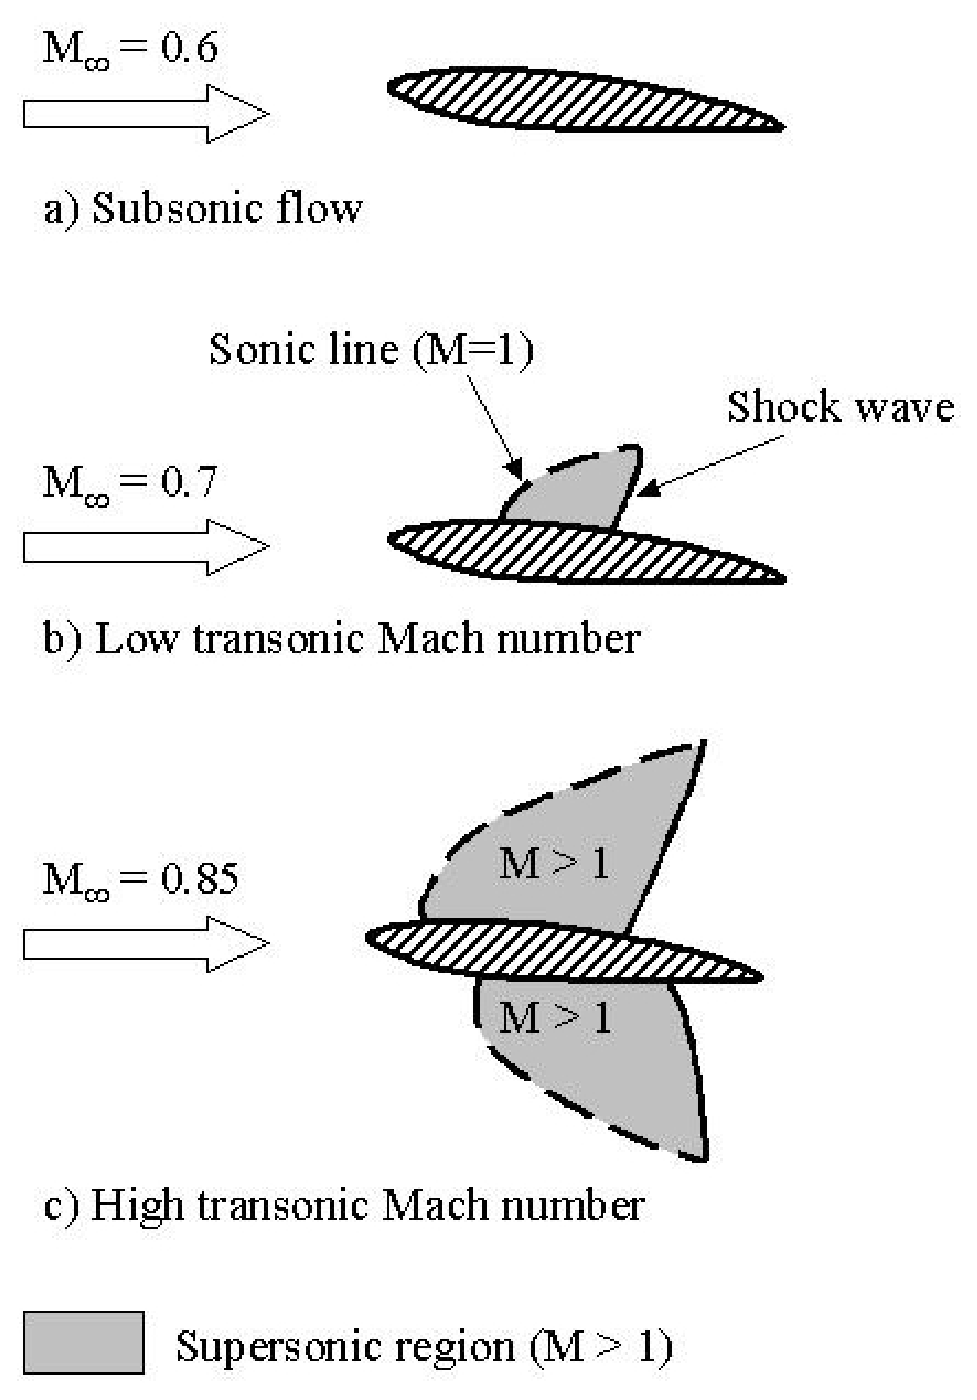
\includegraphics[height=6in]{aflow}
    \else
      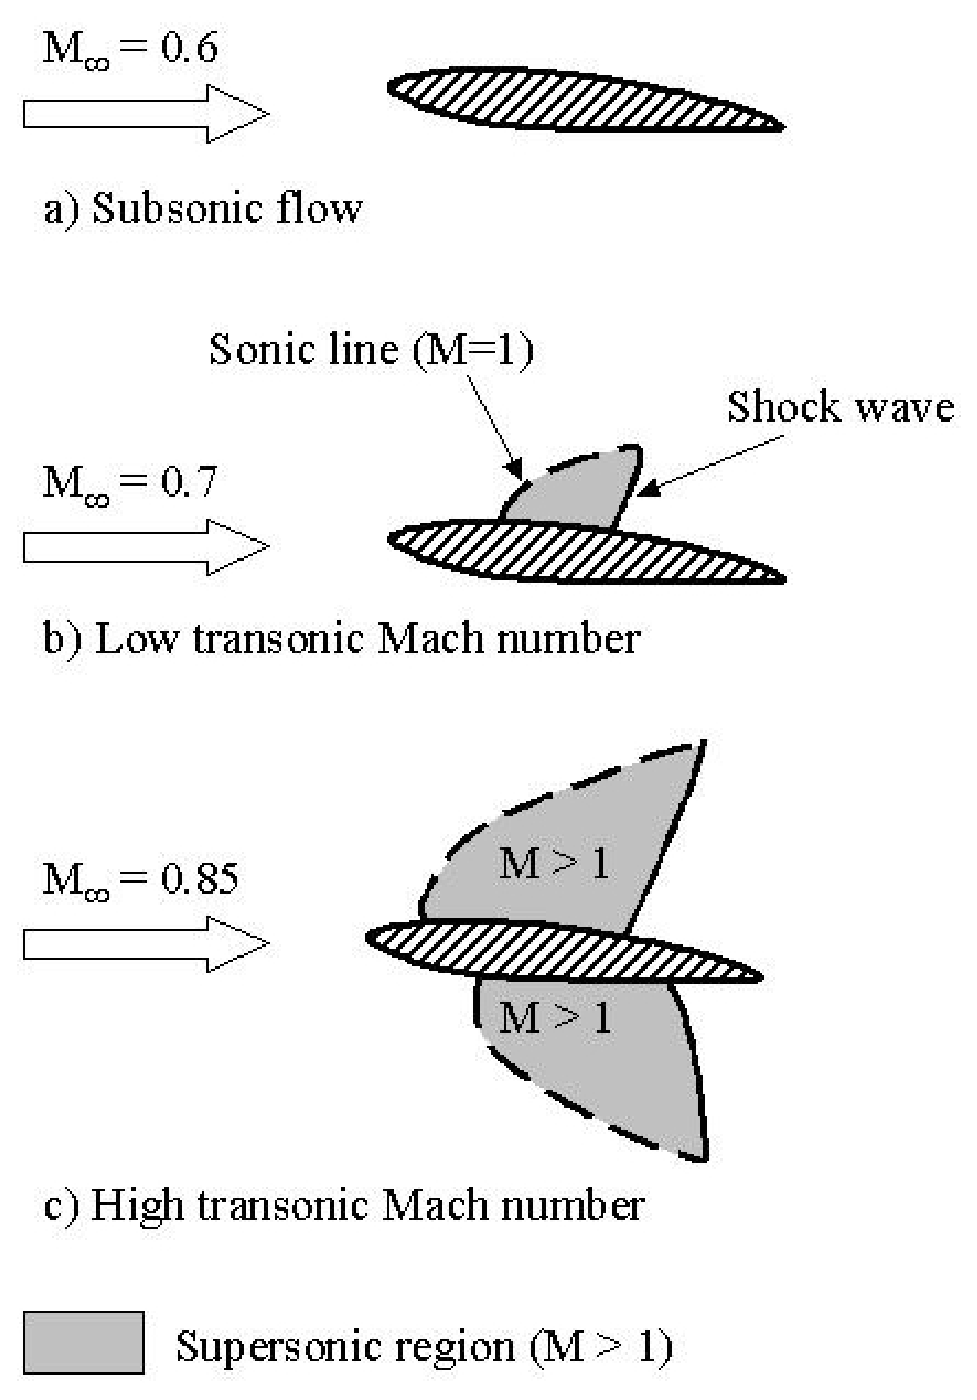
\includegraphics[bb = 92 86 545 742, height=6in]{aflow}
    \fi
    \caption{Airfoil Picture}
    \label{FigAir}
  \end{center}
\end{figure}

% above code has been macro-fied in Classes/MacroFile.tex file
%\InsertFig{\IncludeGraphicsH{aflow}{6in}{92 86 545 742}}{Airfoil Picture}{FigAir}

So as we have now labelled it we can reference it, like so (\ref{FigAir}) and it
is on Page \pageref{FigAir}. And as we can see, it is a very nice picture and we
can talk about it all we want and when we are tired we can move on to the next
chapter ...

I would also like to add an extra bookmark in acroread like so ...
\ifpdf
  \pdfbookmark[2]{bookmark text is here}{And this is what I want bookmarked}
\fi
% ------------------------------------------------------------------------


%%% Local Variables: 
%%% mode: latex
%%% TeX-master: "../thesis"
%%% End: 

\chapter{My Second Chapter}
\ifpdf
    \graphicspath{{Chapter2/Chapter2Figs/PNG/}{Chapter2/Chapter2Figs/PDF/}{Chapter2/Chapter2Figs/}}
\else
    \graphicspath{{Chapter2/Chapter2Figs/EPS/}{Chapter2/Chapter2Figs/}}
\fi

\section{First Section}
\markboth{\MakeUppercase{\thechapter. My Second Chapter }}
And now I begin my second chapter here ...

\section{Second Section}
\markboth{\MakeUppercase{\thechapter. My Second Chapter }}
and here I write more ...

\subsection{first subsection in the Second Section}
... and some more ...

\subsection{second subsection in the Second Section}
... and some more ...

\subsection{third subsection in the Second Section}
... and some more ...

% ------------------------------------------------------------------------

%%% Local Variables: 
%%% mode: latex
%%% TeX-master: "../thesis"
%%% End: 

\chapter{My Third Chapter}
\ifpdf
    \graphicspath{{Chapter3/Chapter3Figs/PNG/}{Chapter3/Chapter3Figs/PDF/}{Chapter3/Chapter3Figs/}}
\else
    \graphicspath{{Chapter3/Chapter3Figs/EPS/}{Chapter3/Chapter3Figs/}}
\fi

\section{First Section of the Third Chapter}
\markboth{\MakeUppercase{\thechapter. My Third Chapter }}{\thechapter. My Third Chapter}
And now I begin my third chapter here ...

\subsection{first subsection in the First Section}
... and some more 

\subsection{second subsection in the First Section}
... and some more ...

\subsubsection{first subsub section in the second subsection}
... and some more in the first subsub section otherwise it all looks the same
doesn't it? well we can add some text to it ...

\subsection{third subsection in the First Section}
... and some more ...

\subsubsection{first subsub section in the third subsection}
... and some more in the first subsub section otherwise it all looks the same
doesn't it? well we can add some text to it and some more and some more and
some more and some more and some more and some more and some more ...

\subsubsection{second subsub section in the third subsection}
... and some more in the first subsub section otherwise it all looks the same
doesn't it? well we can add some text to it ...

\section{Second Section of the Third Chapter}
\markboth{\MakeUppercase{\thechapter. My Third Chapter }}{\thechapter. My Third Chapter}
and here I write more ...

% ------------------------------------------------------------------------


%%% Local Variables: 
%%% mode: latex
%%% TeX-master: "../thesis"
%%% End: 

\def\baselinestretch{1}
\chapter{My Conclusions ...}
\ifpdf
    \graphicspath{{Conclusions/ConclusionsFigs/PNG/}{Conclusions/ConclusionsFigs/PDF/}{Conclusions/ConclusionsFigs/}}
\else
    \graphicspath{{Conclusions/ConclusionsFigs/EPS/}{Conclusions/ConclusionsFigs/}}
\fi

\def\baselinestretch{1.66}

Here I put my conclusions ...

%%% ----------------------------------------------------------------------

% ------------------------------------------------------------------------

%%% Local Variables: 
%%% mode: latex
%%% TeX-master: "../thesis"
%%% End: 


\backmatter % book mode only
\appendix
% ******************************* Thesis Appendix A ****************************
\chapter{How to install \LaTeX} 

\section*{Windows OS}

\subsection*{TeXLive package - full version}
\begin{enumerate}
\item	Download the TeXLive ISO (2.2GB) from\\
\href{https://www.tug.org/texlive/}{https://www.tug.org/texlive/}
\item	Download WinCDEmu (if you don't have a virtual drive) from \\
\href{http://wincdemu.sysprogs.org/download/}
{http://wincdemu.sysprogs.org/download/}
\item	To install Windows CD Emulator follow the instructions at\\
\href{http://wincdemu.sysprogs.org/tutorials/install/}
{http://wincdemu.sysprogs.org/tutorials/install/}
\item	Right click the iso and mount it using the WinCDEmu as shown in \\
\href{http://wincdemu.sysprogs.org/tutorials/mount/}{
http://wincdemu.sysprogs.org/tutorials/mount/}
\item	Open your virtual drive and run setup.pl
\end{enumerate}

or

\subsection*{Basic MikTeX - \TeX~ distribution}
\begin{enumerate}
\item	Download Basic-MiK\TeX (32bit or 64bit) from\\
\href{http://miktex.org/download}{http://miktex.org/download}
\item	Run the installer 
\item	To add a new package go to Start >> All Programs >> MikTex >> Maintenance (Admin) and choose Package Manager
\item	Select or search for packages to install
\end{enumerate}

\subsection*{TexStudio - \TeX~ editor}
\begin{enumerate}
\item	Download TexStudio from\\
\href{http://texstudio.sourceforge.net/\#downloads}
{http://texstudio.sourceforge.net/\#downloads} 
\item	Run the installer
\end{enumerate}

\section*{Mac OS X}
\subsection*{MacTeX - \TeX~ distribution}
\begin{enumerate}
\item	Download the file from\\
\href{https://www.tug.org/mactex/}{https://www.tug.org/mactex/}
\item	Extract and double click to run the installer. It does the entire configuration, sit back and relax.
\end{enumerate}

\subsection*{TexStudio - \TeX~ editor}
\begin{enumerate}
\item	Download TexStudio from\\
\href{http://texstudio.sourceforge.net/\#downloads}
{http://texstudio.sourceforge.net/\#downloads} 
\item	Extract and Start
\end{enumerate}


\section*{Unix/Linux}
\subsection*{TeXLive - \TeX~ distribution}
\subsubsection*{Getting the distribution:}
\begin{enumerate}
\item	TexLive can be downloaded from\\
\href{http://www.tug.org/texlive/acquire-netinstall.html}
{http://www.tug.org/texlive/acquire-netinstall.html}.
\item	TexLive is provided by most operating system you can use (rpm,apt-get or yum) to get TexLive distributions
\end{enumerate}

\subsubsection*{Installation}
\begin{enumerate}
\item	Mount the ISO file in the mnt directory
\begin{verbatim}
mount -t iso9660 -o ro,loop,noauto /your/texlive####.iso /mnt
\end{verbatim}

\item	Install wget on your OS (use rpm, apt-get or yum install)
\item	Run the installer script install-tl.
\begin{verbatim}
	cd /your/download/directory
	./install-tl
\end{verbatim}
\item	Enter command `i' for installation

\item	Post-Installation configuration:\\
\href{http://www.tug.org/texlive/doc/texlive-en/texlive-en.html\#x1-320003.4.1}
{http://www.tug.org/texlive/doc/texlive-en/texlive-en.html\#x1-320003.4.1} 
\item	Set the path for the directory of TexLive binaries in your .bashrc file
\end{enumerate}

\subsubsection*{For 32bit OS}
For Bourne-compatible shells such as bash, and using Intel x86 GNU/Linux and a default directory setup as an example, the file to edit might be \begin{verbatim}
edit $~/.bashrc file and add following lines
PATH=/usr/local/texlive/2011/bin/i386-linux:$PATH; 
export PATH 
MANPATH=/usr/local/texlive/2011/texmf/doc/man:$MANPATH;
export MANPATH 
INFOPATH=/usr/local/texlive/2011/texmf/doc/info:$INFOPATH;
export INFOPATH
\end{verbatim}
\subsubsection*{For 64bit OS}
\begin{verbatim}
edit $~/.bashrc file and add following lines
PATH=/usr/local/texlive/2011/bin/x86_64-linux:$PATH;
export PATH 
MANPATH=/usr/local/texlive/2011/texmf/doc/man:$MANPATH;
export MANPATH 
INFOPATH=/usr/local/texlive/2011/texmf/doc/info:$INFOPATH;
export INFOPATH

\end{verbatim}



%\subsection{Installing directly using Linux packages} 
\subsubsection*{Fedora/RedHat/CentOS:}
\begin{verbatim} 
sudo yum install texlive 
sudo yum install psutils 
\end{verbatim}


\subsubsection*{SUSE:}
\begin{verbatim}
sudo zypper install texlive
\end{verbatim}


\subsubsection*{Debian/Ubuntu:}
\begin{verbatim} 
sudo apt-get install texlive texlive-latex-extra 
sudo apt-get install psutils
\end{verbatim}

% ******************************* Thesis Appendix B ********************************

\chapter{Installing the CUED class file}

\LaTeX.cls files can be accessed system-wide when they are placed in the
<texmf>/tex/latex directory, where <texmf> is the root directory of the user’s \TeX installation. On systems that have a local texmf tree (<texmflocal>), which
may be named ``texmf-local'' or ``localtexmf'', it may be advisable to install packages in <texmflocal>, rather than <texmf> as the contents of the former, unlike that of the latter, are preserved after the \LaTeX system is reinstalled and/or upgraded.

It is recommended that the user create a subdirectory <texmf>/tex/latex/CUED for all CUED related \LaTeX class and package files. On some \LaTeX systems, the directory look-up tables will need to be refreshed after making additions or deletions to the system files. For \TeX Live systems this is accomplished via executing ``texhash'' as root. MIK\TeX users can run ``initexmf -u'' to accomplish the same thing.

Users not willing or able to install the files system-wide can install them in their personal directories, but will then have to provide the path (full or relative) in addition to the filename when referring to them in \LaTeX.



% \bibliographystyle{plainnat}
\bibliographystyle{Classes/CUEDbiblio}
% \bibliographystyle{Classes/jmb}
% \bibliographystyle{Classes/jmb} % bibliography style
\renewcommand{\bibname}{References} % changes default name Bibliography to References
\bibliography{References/references} % References file

\end{document}
